\documentclass[dvipdfmx]{jsarticle}
\usepackage{url}
\usepackage{listings}
\usepackage[dvipdfmx]{graphicx}
\usepackage{here}
\usepackage{ascmac}\usepackage{listings, jlisting, color}
\definecolor{OliveGreen}{rgb}{0.0,0.6,0.0}
\definecolor{Orenge}{rgb}{0.89,0.55,0}
\definecolor{SkyBlue}{rgb}{0.28, 0.28, 0.95}
\lstset{
  language={C++}, % 言語の指定
  basicstyle={\ttfamily},
  identifierstyle={\small},
  commentstyle={\smallitshape},
  keywordstyle={\small\bfseries},
  ndkeywordstyle={\small},
  stringstyle={\small\ttfamily},
  frame={tb},
  breaklines=true,
  columns=[l]{fullflexible},
  numbers=left,
  xrightmargin=0zw,
  xleftmargin=3zw,
  numberstyle={\scriptsize},
  stepnumber=1,
  numbersep=1zw,
  lineskip=-0.5ex,
  keywordstyle={\color{SkyBlue}},     %キーワード(int, ifなど)の書体指定
  commentstyle={\color{OliveGreen}},  %注釈の書体
  stringstyle=\color{Orenge}          %文字列
}

\begin{document}
\title{課題4}
\author{ロボ団マスターコース}
\maketitle

\section{はじめに}
実機を使って動かしてみよう!\\
今回は、ランダムについて勉強しよう!\\
まずは、下のコードを写経しよう。どんな動きをするか確認できたら、課題にとりくんでみよう!\\
\section{ソースコード}
\begin{lstlisting} 
from microbit import *
import random
names = ["Mary", "Yolanda", "Damien", "Alia", "Kushal", "Mei Xiu", "Zoltan" ]
display.scroll(random.choice(names))
\end{lstlisting}

\subsection{問題1}
1から10の数字がランダムで表示されるプログラムを作ろう!
\subsection{問題2}
2個のデジタルサイコロを作ろう!
\subsection{問題3}
LEDライトをつなげてランダムに点滅するプログラムを作ろう!
\subsection{問題4}
三個のLEDライトをつなげてランダムに選んだLEDを光らせるプログラムを作ろう!
\subsection{問題5}
モールス信号一覧→からランダムに文字を選んでLEDでモールス信号を光らせよう!
\begin{figure}[H]
  \centering
  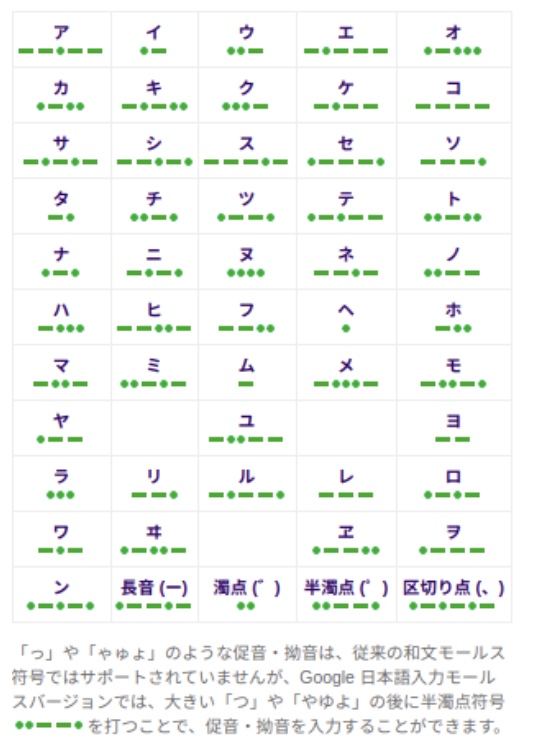
\includegraphics[width=4cm]{1.png}
  \caption{モールス信号早見表}
\end{figure}

\end{document}
